% Created 2020-06-20 Sat 11:36
% Intended LaTeX compiler: pdflatex
\documentclass[11pt]{article}
\usepackage[utf8]{inputenc}
\usepackage[T1]{fontenc}
\usepackage{graphicx}
\usepackage{grffile}
\usepackage{longtable}
\usepackage{wrapfig}
\usepackage{rotating}
\usepackage[normalem]{ulem}
\usepackage{amsmath}
\usepackage{textcomp}
\usepackage{amssymb}
\usepackage{capt-of}
\usepackage{hyperref}
\usepackage[russian]{babel}
\usepackage{esint}
\usepackage{mathtools}
\usepackage{amsthm}
\usepackage[top=0.8in, bottom=0.75in, left=0.625in, right=0.625in]{geometry}
\usepackage{dot2texi}
\usepackage{tikz}
\usetikzlibrary{shapes, arrows, positioning}
\def\zall{\setcounter{Def}{0}\setcounter{lem}{0}\setcounter{cnsqnc}{0}\setcounter{th}{0}\setcounter{Cmt}{0}\setcounter{equation}{0}\setcounter{stnmt}{0}}
\newcounter{Def}\setcounter{Def}{0}
\def\df{\par\smallskip\refstepcounter{Def}\textbf{\arabic{Def}}}
\newtheorem*{Def}{Определение \df}
\newcounter{lem}\setcounter{lem}{0}
\def\lm{\par\smallskip\refstepcounter{lem}\textbf{\arabic{lem}}}
\newtheorem*{Lemma}{Лемма \lm}
\newcounter{th}\setcounter{th}{0}
\def\th{\par\smallskip\refstepcounter{th}\textbf{\arabic{th}}}
\newtheorem*{Theorem}{Теорема \th}
\newcounter{cnsqnc}\setcounter{cnsqnc}{0}
\def\cnsqnc{\par\smallskip\refstepcounter{cnsqnc}\textbf{\arabic{cnsqnc}}}
\newtheorem*{Consequence}{Следствие \cnsqnc}
\newcounter{Cmt}\setcounter{Cmt}{0}
\def\cmt{\par\smallskip\refstepcounter{Cmt}\textbf{\arabic{Cmt}}}
\newtheorem*{Note}{Замечание \cmt}
\newcounter{stnmt}\setcounter{stnmt}{0}
\def\st{\par\smallskip\refstepcounter{stnmt}\textbf{\arabic{stnmt}}}
\newtheorem*{Statement}{Утверждение \st}
\author{Макаров Сергей, группа 327, вариант 3}
\date{\today}
\title{Экзамен по предмету "Основы кибернетики"}
\hypersetup{
 pdfauthor={Макаров Сергей, группа 327, вариант 3},
 pdftitle={Экзамен по предмету "Основы кибернетики"},
 pdfkeywords={},
 pdfsubject={},
 pdfcreator={Emacs 28.0.50 (Org mode 9.3)}, 
 pdflang={Russian}}
\begin{document}

\maketitle
\pagestyle{myheadings}
\markright{Макаров Сергей, группа 327, вариант 3}

\section{Вопрос 1}
\label{sec:org3970b25}
\zall  
\begin{enumerate}
\item Определение соседних наборов куба.
\item Формулировка критерия единственности ДНФ для булевой функции от \(n\) переменных и следствия из него для линейных булевых функций
\end{enumerate}
\subsection{Ответ}
\label{sec:org445ed80}
   \begin{Def}
Наборы булева куба $B^n$ называются \textbf{соседними по переменной $x_i$}, если они отличаются только в этой переменной.
   \end{Def}
\begin{Def}
Множество $N_f = \{\alpha | f(\alpha) = 1\}$ называется \textbf{характеристическим множеством} ФАЛ $f$. Функция $f$ называется \textbf{характеристической функцией этого множества}.
\end{Def}
\begin{Lemma}
Совершенная ДНФ ФАЛ $f$ от $n$ БП $x_1, \ldots, x_n$ является единственной ДНФ, реализующей эту функцию тогда и только тогда, когда в её характеристическом множестве нет соседним наборов.
\end{Lemma}
\begin{Consequence}
Совершенные ДНФ функций $l_n = x_1 \oplus \ldots \oplus x_n$ и $\overline{l}_n = x_1 \oplus \ldots \oplus x_n \oplus 1$ являются единственными ДНФ этих функций, т. к. на всех соседних наборах эти функции принимают противоположные значения.
\end{Consequence}
\pagebreak
\section{Вопрос 2}
\label{sec:orgd6124a7}
\zall  
\begin{enumerate}
\item Формулировка утверждения о длине градиентного покрытия матрицы с заданной долей единиц в её столбцах.
\item Идея его доказательства
\end{enumerate}
\subsection{Ответ}
\label{sec:org8dee76a}
   \begin{Theorem}
Пусть для $\gamma \in (0, 1]$ в каждом столбце матрицы $M \in B^{p \times s}$ имеется не меньше, чем $\gamma\cdot p$ единиц. Тогда покрытие матрицы $M$, получаемое с помощью градиентного алгоритма, имеет длину не больше, чем $\lceil\frac1{\gamma}\ln^+(\gamma s)\rceil + \frac1{\gamma}$, где $\ln^+ x = \max(\ln x, 0)$.
   \end{Theorem}
   \begin{proof}
Пусть построение градиентного покрытия матрицы $M$ потребовало $q$ шагов, и на $t$-м шаге была выбрана строка с номером $i_t$. Рассмотрим матрицу $M_t$, полученную в результате удаления всех строк, выбранных на шагах до $t$-го включительно, и покрытых ими столбцов. $M \in B^{p_t\times s_t}, p_t = p - t, s_t = s\cdot \delta_t, \delta_t \in [0, 1]$. Положим также $M_0 = M, p_0 = p, s_0 = s, \delta_0 = 1$  и $s_q = \delta_q = 0$. При любом $t = \overline{0, q}$ справедливо неравенство:
\begin{equation}\label{neq:2-1}
q \leq t + \delta_t\cdot s,
\end{equation}
поскольку после первых $t$ шагов алгоритма остаются не покрытыми $\delta_t\cdot s$ столбцов $M$, при этом на каждом последующем шаге покрывается как минимум один столбец.

Поскольку в каждом столбце матрицы имеется не менее, чем $\gamma\cdot p$ единиц, то общее число единиц в матрице $M_t$ как минимум $\gamma ps\delta_t$, из чего следует, что в среднем в каждой строке не меньше, чем $\gamma s\delta_t$ единиц. Поскольку на каждом шаге выбирается строка с максимальным числом единиц, строка с номером $i_{t + 1}$ содержит по крайней мере $\gamma s\delta_t$ единиц, т. е. покрывает по крайней мере $\gamma s\delta_t$ столбцов. Это обеспечивает выполнение соотношений:
\begin{equation*}
s\delta_{t + 1} = s_{t + 1} \leq s_t - \gamma s\delta_t = s\delta_t(1 - \gamma)\, \forall t = \overline{0, q - 1}
\end{equation*}
из чего следует, что
\begin{equation}\label{neq:2-2}
\delta_t \leq (1 - \gamma)^t \leq e^{-\gamma t}
\end{equation}
Выбрав $t = \lceil\frac1{\gamma}\ln^+(\gamma s)\rceil$ и используя \eqref{neq:2-1} и \eqref{neq:2-2}, получаем:
\begin{equation}
q \leq \lceil\frac1{\gamma}\ln^+(\gamma s)\rceil + s\cdot e^{ln^+(\gamma s)} \leq \lceil\frac1{\gamma}\ln^+(\gamma s)\rceil + \frac1{\gamma},
\end{equation}
что и требовалось доказать.
   \end{proof}
\pagebreak
\section{Вопрос 3}
\label{sec:org0a22519}
\zall
\begin{enumerate}
\item Определение изоморфных и эквивалентных КС.
\item Верхняя оценка числа попарно неэквивалентных (1, 1)-КС от булевых переменных \(x_1, \ldots, x_n\), имеющих сложность не больше, чем \(L\).
\end{enumerate}
\subsection{Ответ}
\label{sec:org7de6af1}
   \begin{Def}
Контактные схемы $\Sigma_1$ и $\Sigma_2$ называются \textbf{изморфными}, если изоморфны 
графы, соответствующие этим схемам.
   \end{Def}
\begin{Def}
Контактные схемы $\Sigma_1$ и $\Sigma_2$ называются \textbf{эквивалентными}, если они реализуют равные системы ФАЛ, т. е. функции проводимости между соответствующими парами входов и выходов совпадают.
\end{Def}
\begin{Def}
КС $(1, m)$ называется \textbf{приведённой}, если все её изолированные вершины являются полюсами, а все контакты и остальные вершины этой схемы лежат на простых проводящих цепях, соединяющих её вход и выходы.
\end{Def}
Обозначим через $U^K(L, n)$ множество приведённых $(1, 1)$-схем, сложность которых не выше $L$. Через $||U||$ будем обозначать число попарно неэквивалентных схем в классе $U$. Заметим, что каждая неприведённая схема $\Sigma$ эквивалентна приведённой схеме, полученной из $\Sigma$ удалением изолированных вершин, не являющихся полюсами и контактов и вершин, не лежащих на простых проводящих цепях, соединяющих её вход и выходы.
\begin{Lemma}
$\forall L, n \in \mathbb{N}$:
\begin{equation*}
||U^K(L, n)|| \leq (8nL)^L
\end{equation*}
\end{Lemma}
\pagebreak
\section{Вопрос 4}
\label{sec:org6d1fa0a}
\zall
\begin{enumerate}
\item Обобщённое тождество \(t_4^{(n)}\) для ЭП КС.
\item Идея его вывода из основных или других обобщённых тождеств.
\item Описать тот этап приведения КС от БП \(x_1, \ldots, x_n\) к каноническому виду, на котором используется данное тождество.
\end{enumerate}
\subsection{Ответ}
\label{sec:org8e7682a}
\pagebreak
\section{Вопрос 5}
\label{sec:orgc3ad3ac}
\zall
\begin{enumerate}
\item Мультиплексорная булева функция \(\mu_n\) порядка \(n\).
\item Формулировка утверждения о верхней оценке сложности её реализации в классе \(\pi\)-схем.
\item Идея его доказательства
\end{enumerate}
\subsection{Ответ}
\label{sec:orgca68cd6}
   \begin{Def}
Функция вида
\begin{equation*}
\mu_n(x_1, \ldots, x_n, y_0, \ldots, y_{2^n - 1}) = \bigvee\limits_{\alpha = (\alpha_1, \ldots, \alpha_n)}x_1^{\alpha_1}\ldots x_n^{\alpha_n}y_{\nu(\alpha)}
\end{equation*}
называется \textbf{мультиплексорной функцией} или \textbf{мультиплексором порядка $n$}. Переменные $x_1, \ldots, x_n$ называются \textbf{адресными}, а $y_1, \ldots, y_{2^n - 1}$, соответственно, \textbf{информационными}.
   \end{Def}
\begin{Lemma}
\begin{equation*}
\forall n \in \mathbb{N}: L^{\pi}(\mu_n) \leq 3\cdot2^n - 2.
\end{equation}
\end{Lemma}
\begin{proof}
Данная оценка получается посредством использования следующей схемы:
\begin{figure}[h]
\begin{center}
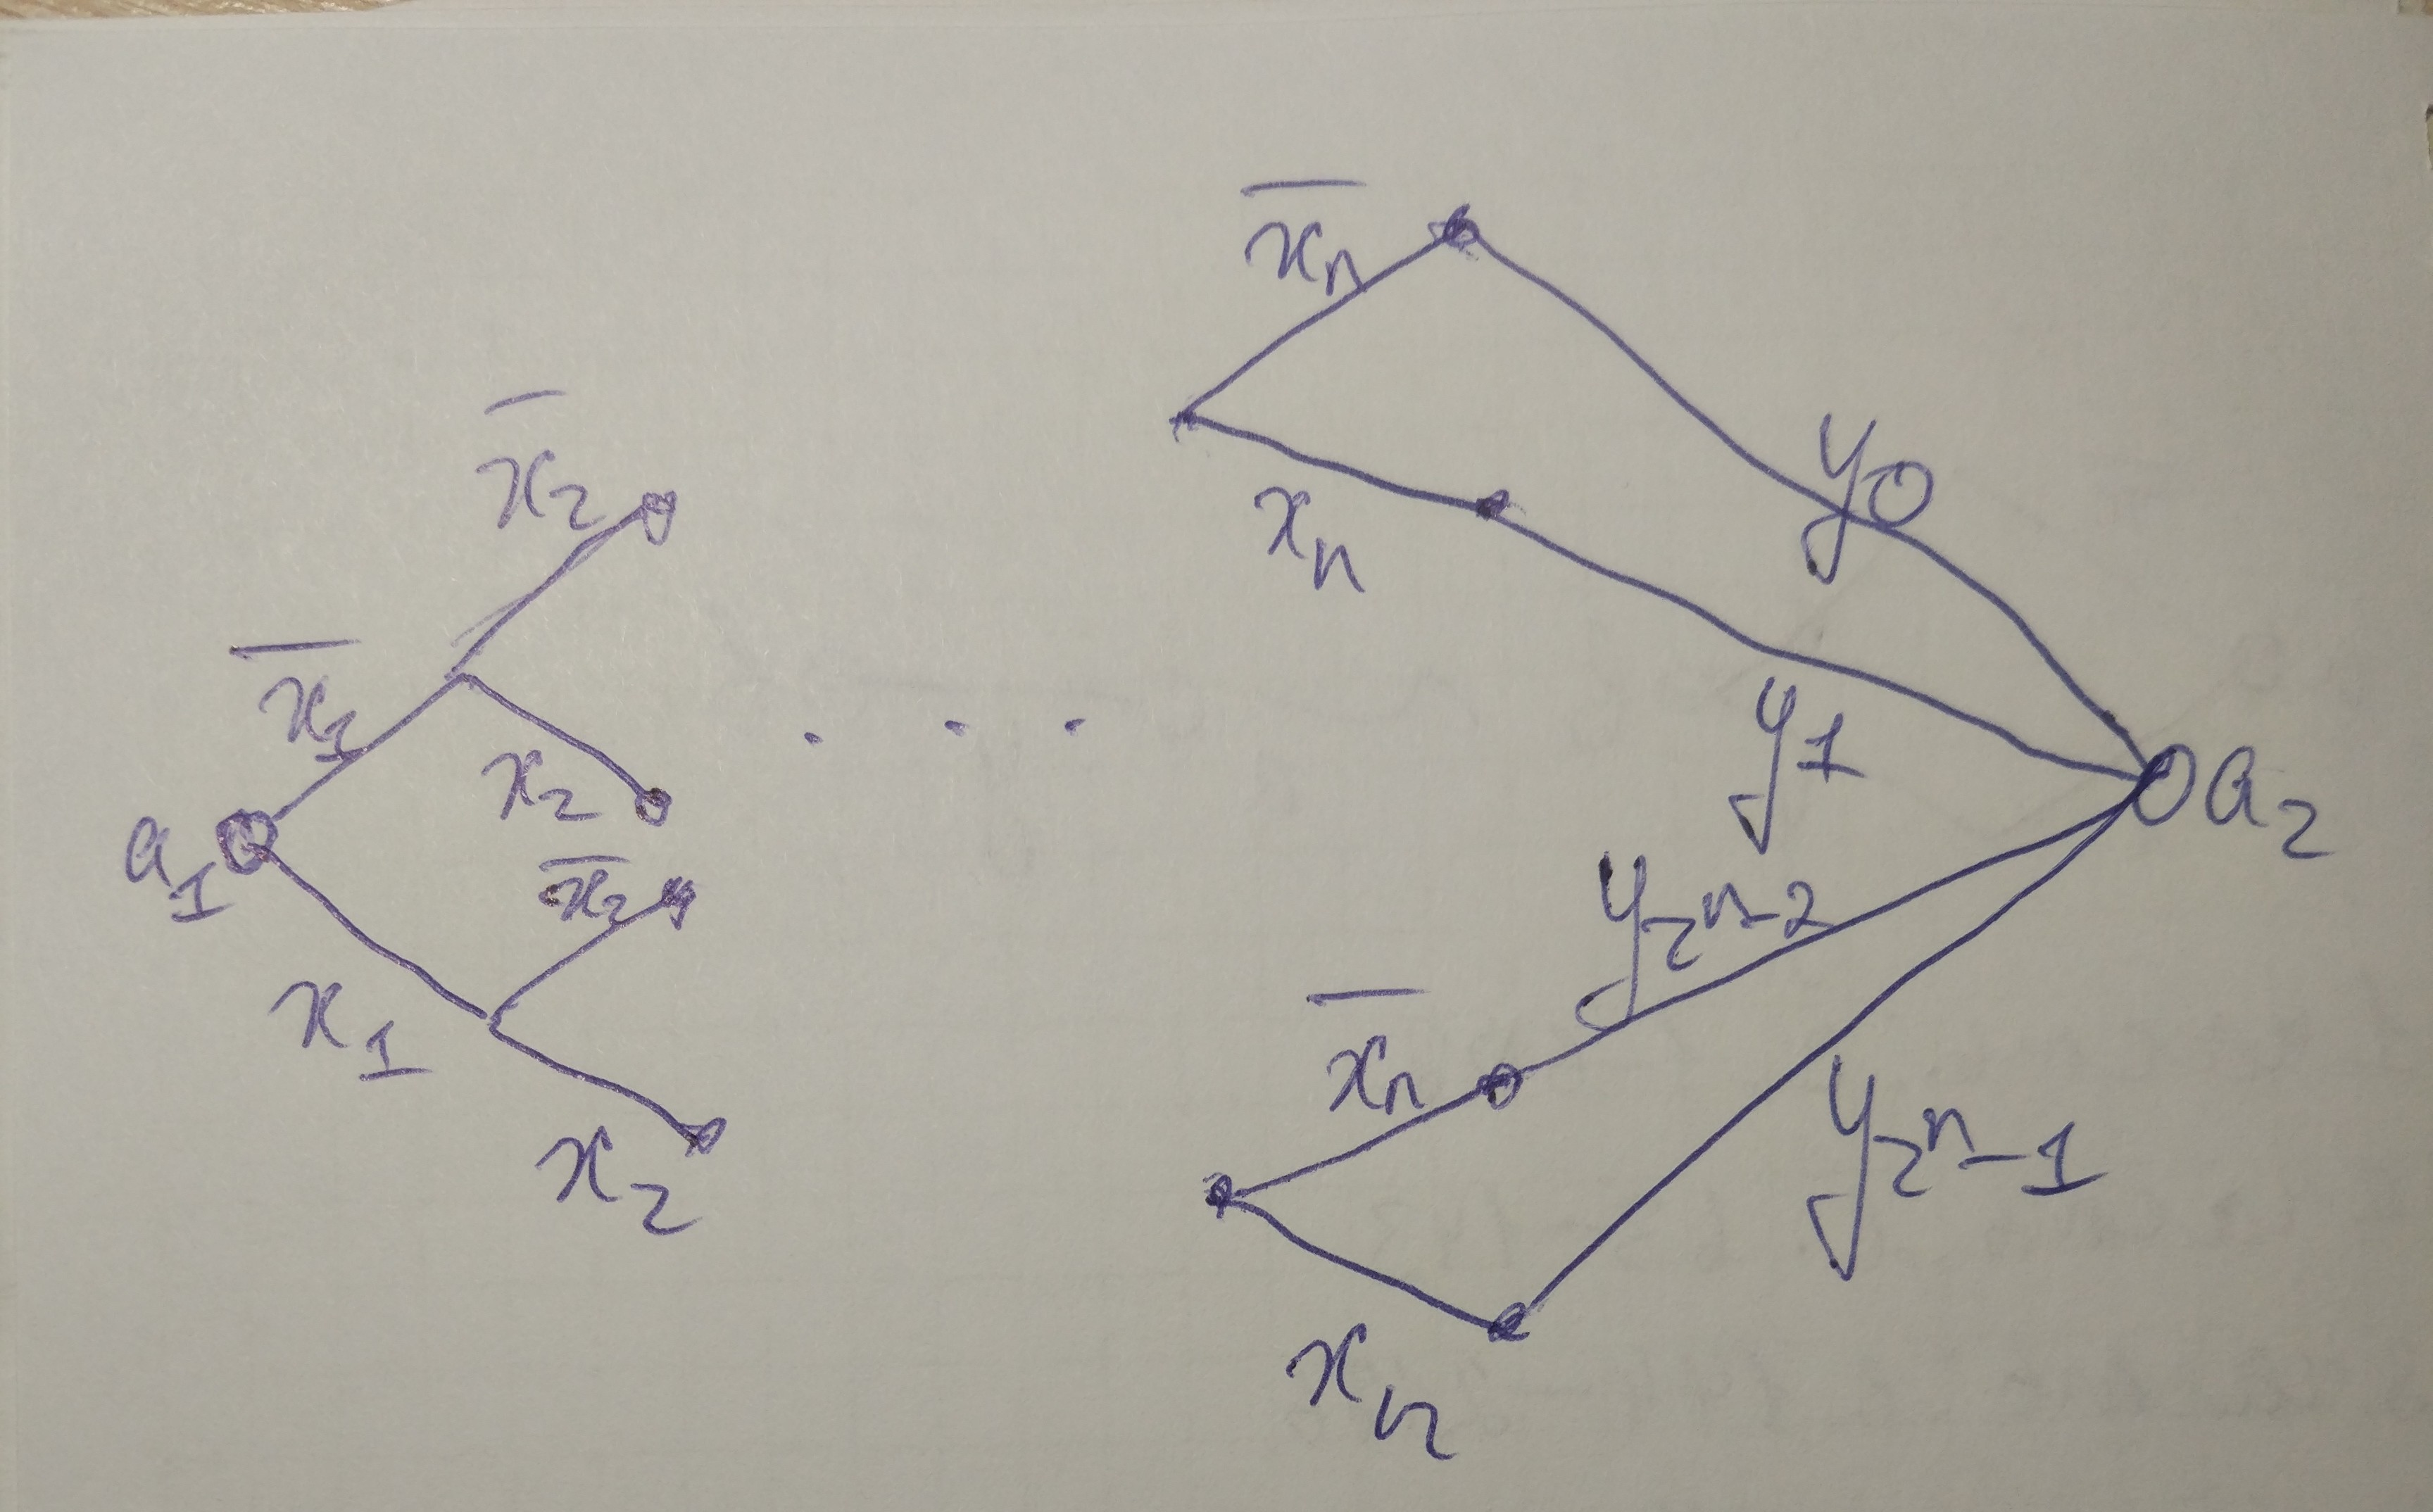
\includegraphics[width=.9\linewidth]{./scheme1.jpg}
\end{center}
\end{figure}
\end{proof}
\pagebreak
\section{Вопрос 6}
\label{sec:org425b54d}
\zall
\begin{enumerate}
\item Определения сложности реализации булевой функции контактными схемами и функции Шеннона сложности КС.
\item Утверждение о сложности КС, получаемых асимптотически наилучшим методом синтеза, и вытекающие из него верхние оценки соответствующей функции Шеннона.
\end{enumerate}
\subsection{Ответ}
\label{sec:org0287d00}
   \begin{Def}
   \textbf{Сложностью реализации БФ $f$ контактными схемами} называется функция:
\begin{equation*}
L^K(f) = \min_{\Sigma \text{ реализует } f}L(\Sigma)
\end{equation*}
   \end{Def}
   \begin{Def}
    \textbf{Функция Шеннона} для сложности КС, реализующих функции от БП $x_1, \ldots, x_n$:
    \begin{equation*}
        L^K(n) = \max_{f \in P_2(n)} L^K(f)
    \end{equation*}
\end{Def}
\begin{Theorem}
    Для любой ФАЛ $f \in P_2(n)$ существует реализующая её КС $\Sigma_f$ такая, что:
    \begin{equation}\label{eq:ks-compl}
        L(\Sigma_f) \leq \frac{2^n}n\left(1 + O\left(\frac1{\sqrt{n}}\right)\right)
    \end{equation}
\end{Theorem}
\begin{Consequence}
Из \eqref{eq:ks-compl} следует верхняя оценка для функции Шеннона:
\begin{equation*}
L^K(n) \lesssim \frac{2^n}n
\end{equation*}
\end{Consequence}
\pagebreak
\section{Вопрос 7}
\label{sec:orgab48943}
\zall
\begin{enumerate}
\item Определение теста для отделимой по столбцам матрицы \(M \in B^{p\times s}\) и цели контроля \(\mathcal{N}\), понятие тупикового теста.
\item Определение функции \(F(y_1, \ldots, y_p)\) теста для пары \((M, \mathcal{N})\) и утверждение о представлении данной ФАЛ в виде КНФ.
\end{enumerate}
\subsection{Ответ}
\label{sec:orgabf4ce5}
   \begin{Def}
    \textbf{Целью контроля} для отделимой по столбцам таблицы $M$ называется множество $\mathcal{N}$, состоящее из неупорядоченных пар различных чисел отрезка $[1, s]$, для которых пары столбцов матрицы с соответствующими номерами необходимо отличать.
\end{Def}
\begin{Def}
    Множество строк матрицы $M$ с номерами из $T, T \subseteq [1, p]$ называется \textbf{тестом для матрицы $M$ относительно множества $\mathcal{N}$} или \textbf{тестом для} $(M, \mathcal{N})$, если $\forall i, j \in \mathcal{N} \exists t \in T: M_{ti} = M_{tj}$. Мощность теста так же называется его \textbf{длиной}.
\end{Def}
\begin{Def}
    Тест для $(M, \mathcal{N})$ называется \textbf{тупиковым}, если он перестаёт быть тестом при удалении любой своей строки.
\end{Def}
\begin{Def}
    Пусть $M$ -- отделимая по столбцам матрица, а $\mathcal{N}$ -- связанная с ней цель контроля. Сопоставим $i$-й строке, $i \in [1, p]$ матрицы БП $y_i$, а каждому набору $\beta \in B^p$ этих переменных -- множество строк матрицы $M$ с номерами из множества $I = I(\beta) \subseteq [1, p]$, где $i \in I(\beta) \Leftrightarrow \beta_i = 1$. Рассмотрим ФАЛ $F(y)$, для которой $F(\beta) = 1$ тогда и только тогда, когда система строк матрицы $M$ с номерами из $I(\beta)$ образует тест для $(M, \mathcal{N})$. Эта ФАЛ называется \textbf{функцией теста для $(M, \mathcal{N})$}.
\end{Def}
\begin{Lemma}
    Функция теста $f(y_1, \ldots, y_p)$ для отделимой по столбцам матрицы $M \in B^{p\times s}$ и цели контроля $\mathcal{N}$ может быть задана с помощью КНФ
    \begin{equation}\label{eq:knf-test}
        f(y_1, \ldots, y_p) = \bigwedge\limits_{(i, j) \in \mathcal{N}}\left(\bigvee\limits_{\substack{1 \leq t \leq p \\ M_{ti} \neq M_{tj}}}y_t\right)
    \end{equation}
\end{Lemma}
\begin{Consequence}
    Каждая ЭК вида $y_1\ldots y_{t_r}$ сокращённой ДНФ $f(y_1, \ldots, y_p)$, получающаяся из КНФ \eqref{eq:knf-test} в результате раскрытия скобок и приведения подобных, соответствует тупиковому тесту, связанному с множеством $T = \{t_1, \ldots, t_r\}$ и обратно.
\end{Consequence}
\pagebreak
\section{Задача 1}
\label{sec:org1951eda}
\zall
Построить сокращённую ДНФ булевой функции \(f(x_1, x_2, x_3, x_4)\), столбец значений которой имеет вид \(\widetilde{\alpha}_f = (0110\, 0011\, 1001\, 0111)\).
\subsection{Решение}
\label{sec:org30fd0d9}
Построим карту Карно для \(f\):
\begin{center}
\begin{tabular}{rrrrr}
\hline
\(x_1x_2\backslash x_3x_4\) & 00 & 01 & 11 & 10\\
\hline
00 & 0 & 1 & 0 & 1\\
01 & 0 & 0 & 1 & 1\\
11 & 0 & 1 & 1 & 1\\
10 & 1 & 0 & 1 & 0\\
\hline
\end{tabular}
\end{center}
Получаем максимальные грани \((1000), (0001), (1121), (2112), (1211), (0210)\).
Такому покрытию \(N_f\) максимальными гранями соответствует сокращённая ДНФ:
\begin{equation*}
f(x_1, x_2, x_3, x_4) = x_1\overline{x}_2\overline{x}_3\overline{x}_4\lor \overline{x}_1\overline{x}_2\overline{x}_3x_4\lor x_1x_2x_4\lor x_2x_3\lor x_1x_3x_4\lor \overline{x}_1x_3\overline{x}_4
\end{equation*}
\pagebreak
\section{Задача 2}
\label{sec:org11f6972}
\zall
С помощью расширенной системы основных тождеств \(\tilde{\tau}^{\text{осн}}\) привести к каноническому виду формулу \(\mathcal{F}\):
\begin{equation}
\mathcal{F} = (\overline{x}_1\lor x_2x_3\lor \overline{x}_2\overline{x}_3)(\overline{x}_2\lor (x_1\lor \overline{x}_3)(\overline{x}_1\lor x_3))
\end{equation}
\subsection{Решение}
\label{sec:orgf2fb870}
\begin{multline*}
\mathcal{F} = (\overline{x}_1\lor x_2x_3\lor \overline{x}_2\overline{x}_3)(\overline{x}_2\lor (x_1\lor \overline{x}_3)(\overline{x}_1\lor x_3)) =^{(4)(D_{\&, \lor})} (\overline{x}_1\lor x_2x_3\lor \overline{x}_2\overline{x}_3)(\overline{x}_2\lor x_1\overline{x}_1\lor \overline{x}_3\overline{x}_1\lor x_1x_3\lor \overline{x_3}x_3) =^{(9)(\text{ПК}_0)} \\
= (\overline{x}_1\lor x_2x_3\lor \overline{x}_2\overline{x}_3)(\overline{x}_2\lor \overline{x}_1\overline{x}_3\lor x_1x_3) =^{(4), (D_{\&, \lor}), \text{ОП}} \\
= \overline{x}_1\overline{x}_2\lor\overline{x}_2\overline{x}_3\lor \overline{x}_1\overline{x}_3\lor x_1x_2x_3
\end{multline*}
\pagebreak
\section{Задача 3}
\label{sec:org3b2b376}
\zall
С помощью метода каскадов, последовательно разлагая булевы функции по переменным \(x_1, x_2, x_3, x_4\), построить (1, 1)-КС \(\Sigma\) для функции \(f(x_1, x_2, x_3, x_4)\), вектор значений которой имеет вид \((0001\, 1001\, 1001\, 1000)\).
\subsection{Решение}
\label{sec:orgb5b01ab}
Построим разложение Шеннона для функции \(f\):
\begin{gather*}
f = \overline{x}_1f_0\lor x_1f_1, f_0 = (0001\,1001), f_1 = (1001\,1000), \\
f_0 = \overline{x}_2f_{00}\lor x_2f_{01}, f_{00} = (0001), f_{01} = (1001), \\
f_1 = \overline{x}_2f_{10}\lor x_2f_{11}, f_{10} = (1001) = f_{01}, f_{11} = (1000), \\
f_{00} = x_3f_{001}, f_{001} = x_4, \\
f_{01} = f_{10} = \overline{x}_3f_{010}\lor x_3f_{011}, f_{010} = \overline{x}_4, f_{011} = x_4, \\
f_{11} = \overline{x}_3f_{110}, f_{110} = \overline{x}_4
\end{gather*}
Соответствующая ККС:
\begin{figure}[h]
\centering
\begin{center}
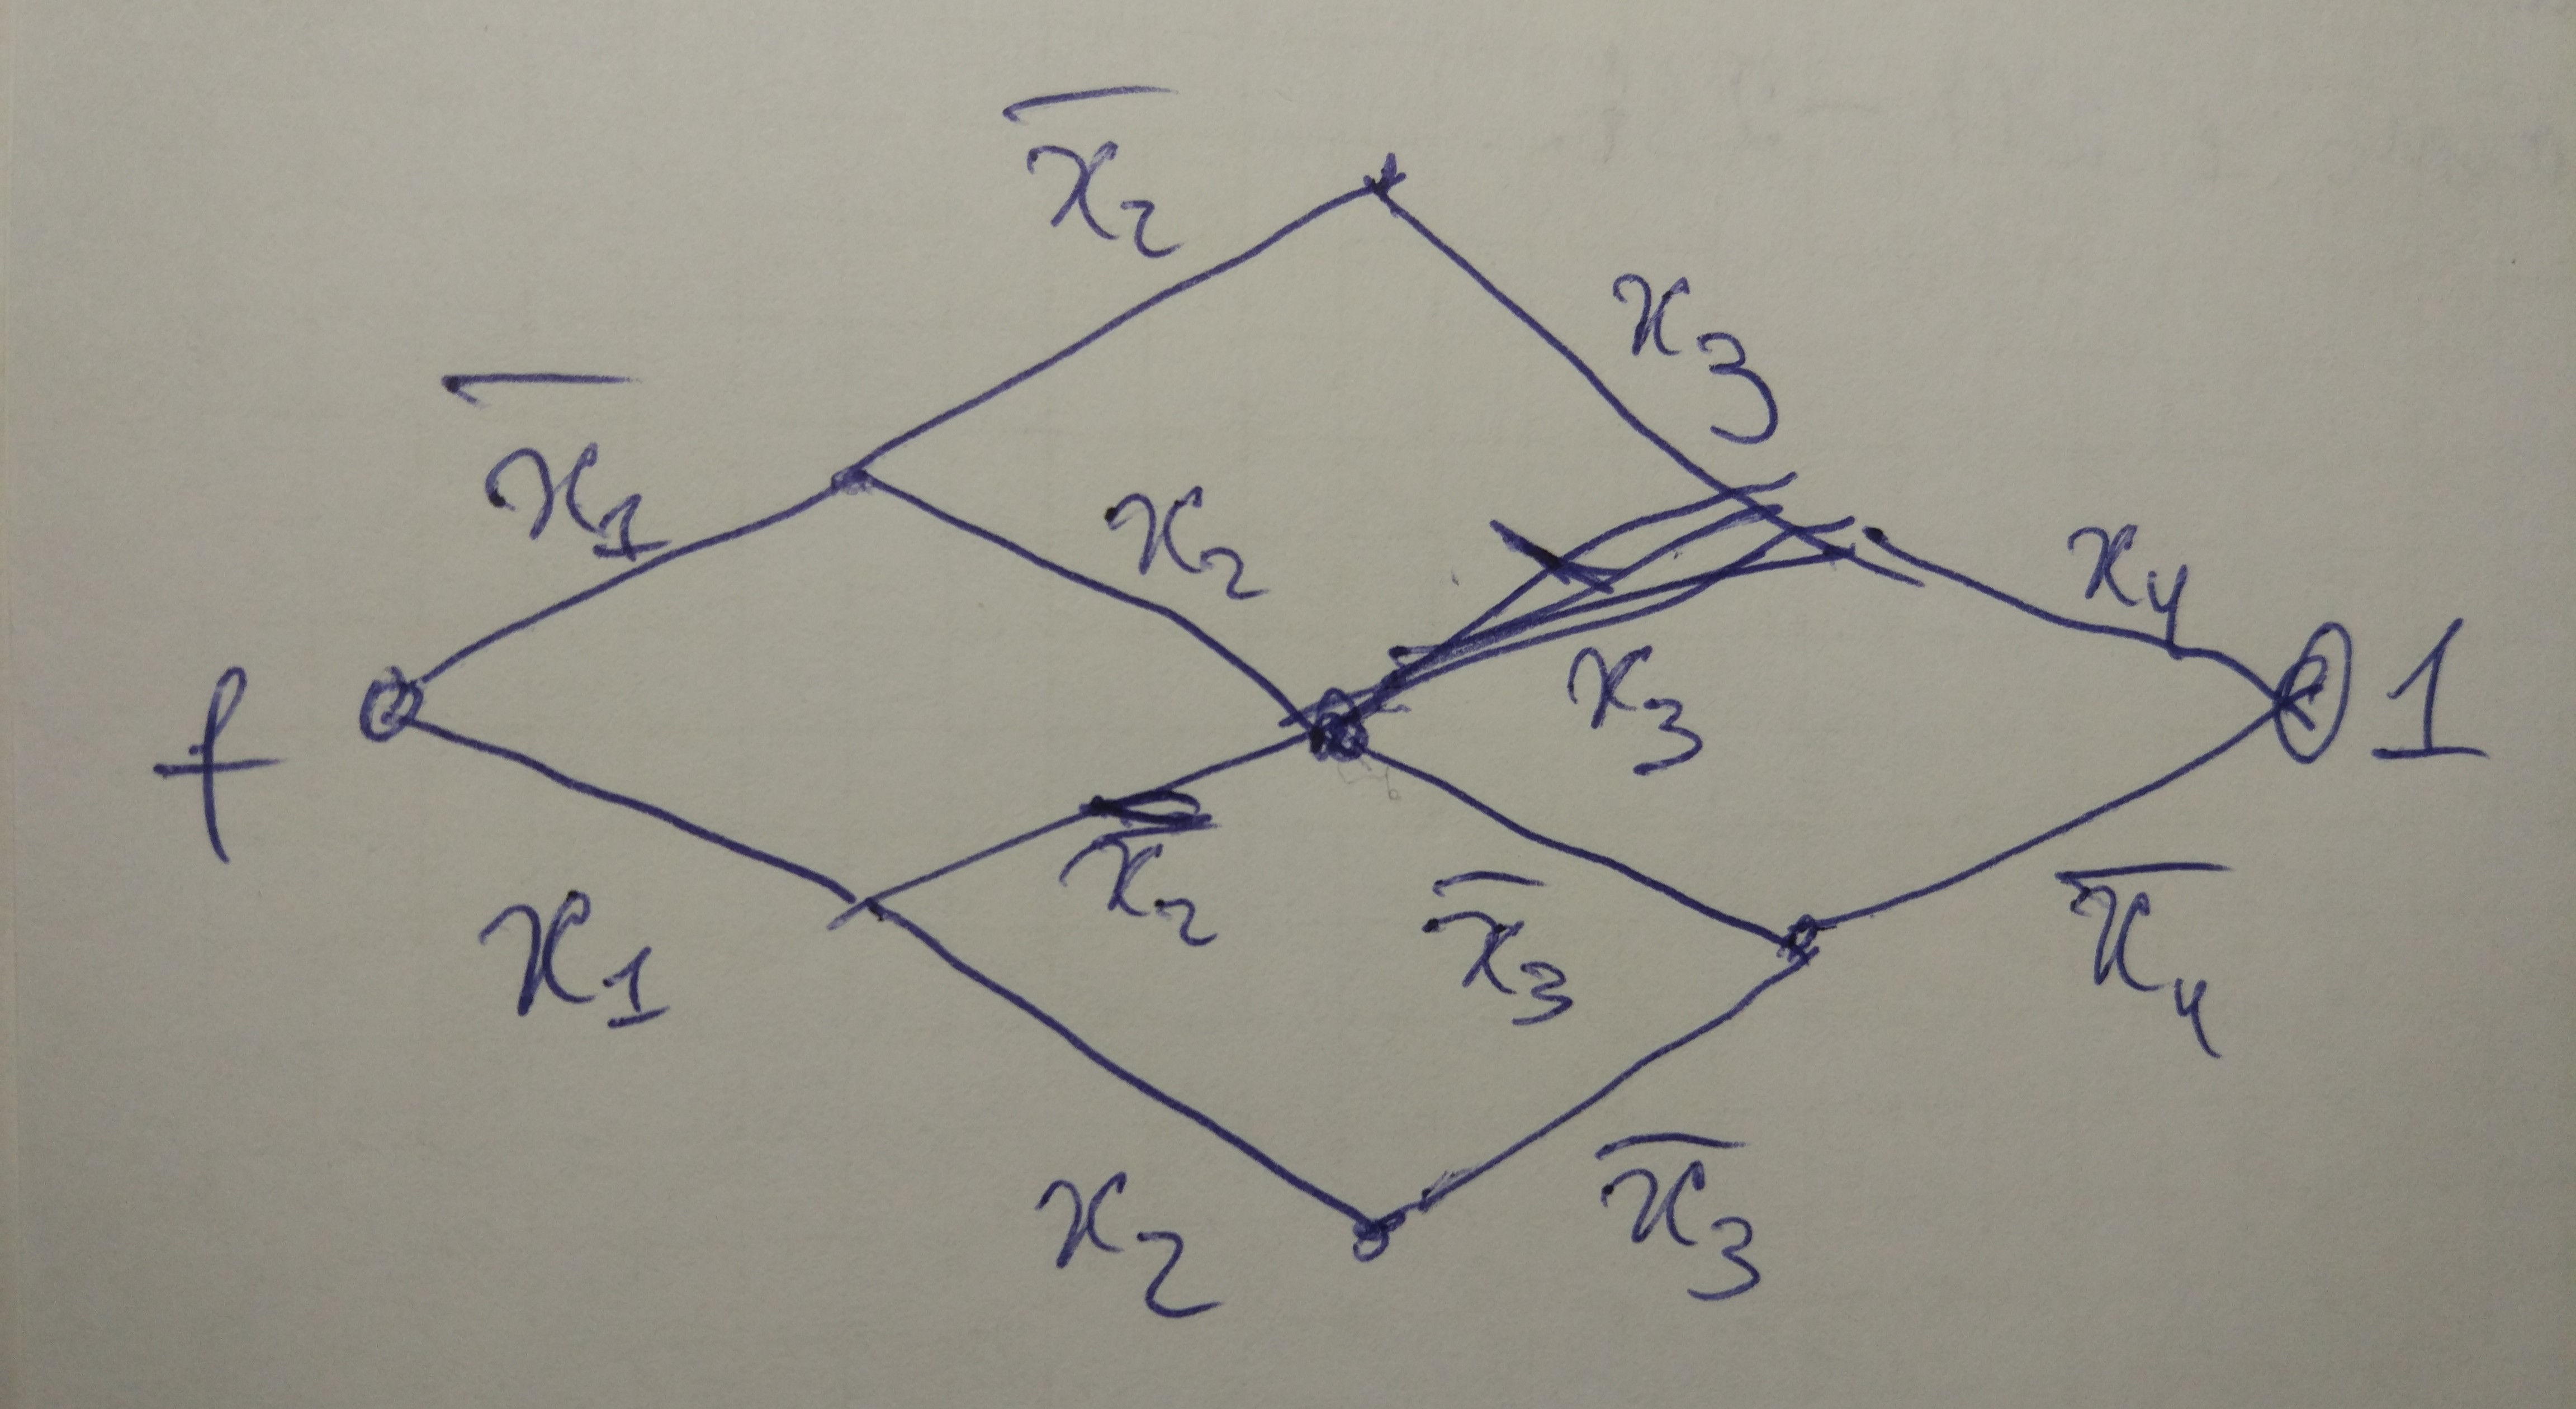
\includegraphics[width=.9\linewidth]{./scheme2.jpg}
\end{center}
\end{figure}
\pagebreak
\end{document}
